\documentclass[aspectratio=169]{beamer}

%%% Работа с русским языком
\usepackage{cmap}					% поиск в PDF
\usepackage{mathtext} 				% русские буквы в формулах
\usepackage[T2A]{fontenc}			% кодировка
\usepackage[utf8]{inputenc}			% кодировка исходного текста
\usepackage[english,russian]{babel}	% локализация и переносы
\usepackage{indentfirst}
\frenchspacing

%%% Дополнительная работа с математикой
\usepackage{amsmath,amsfonts,amssymb,amsthm,mathtools}  % AMS

%%% Текст в колонки
\usepackage{multicol}

%%% Системы уравнений
\usepackage{cases}

%%% Таблицы
\usepackage{array}

%%% Картинки
\usepackage{graphicx}
\usepackage{float}

%%% Гиперссылки
\usepackage{hyperref}

%%% Перенос знаков в формулах (по Львовскому)
\newcommand*{\hm}[1]{#1\nobreak\discretionary{}
{\hbox{$\mathsurround=0pt #1$}}{}}


%%% Свои команды

\newcommand*{\No}{\textnumero}

\newcommand{\vect}[1]{\textbf{\textit{#1}}}
\newcommand{\vx}{{\vect{x}}}

\newcommand{\avphi}{{\widetilde{\phi}}}

\newcommand{\half}{\cfrac{1}{2}}

\newcommand{\partt}[1]{\cfrac{\partial #1}{\partial t}}
\newcommand{\partx}[1]{\cfrac{\partial #1}{\partial x}}
\newcommand{\partxx}[1]{\cfrac{\partial^2 #1}{\partial x^2}}
\newcommand{\partr}[1]{\cfrac{\partial #1}{\partial r}}

\newcommand{\gradscalsq}[1]{\left( \nabla #1, \nabla #1 \right)}

\newcommand{\Natural}{{\mathbb{N}}}
\newcommand{\Real}{{\mathbb{R}}}
\newcommand{\bigO}{{\mathcal{O}}}
\newcommand{\clOmega}{{\overline{\Omega}}}

\newcommand{\norm}[1]{\| #1 \|}
\newcommand{\enorm}{{\| \cdot \|}}

\newcommand{\plapl}[2]{\Div(\norm{\nabla #1}_2^{#2} \nabla #1)}
\newcommand{\bilapl}[1]{\Delta^2 #1}

\newcommand{\gridfunc}[1]{\left[ #1 \right]}


%%% Свои операторы
\DeclareMathOperator{\Div}{{div}}
\DeclareMathOperator{\Const}{{const}}

%%% Цвета
\definecolor{green}{RGB}{0,200,0}
\definecolor{red}{RGB}{200,0,0}

%%% Тема оформления
\usetheme{Madrid}


%%% Титульный лист
\title[Электрический пробой]{Моделирование канала электрического пробоя \\ методом диффузной границы}
\author[]{
	\raggedright
	\hfill \break
	\hspace*{8cm}
	\textbf{Студент:} \linebreak
	\hspace*{8cm}
	\vspace{0.2cm}
	Пономарев Андрей Сергеевич \linebreak
	\hspace*{8cm}
	\textbf{Научный руководитель:} \linebreak
	\hspace*{8cm}
	\vspace{0.2cm}
	Савенков Евгений Борисович
	\hspace*{8cm}
	\textbf{Консультант:} \linebreak
	\hspace*{8cm}
	Зипунова Елизавета Вячеславовна
}
\date{19.11.2024}
\logo{
\includegraphics[height=0.8cm]{../figures/labels.jpg}}


\begin{document}

\begin{frame}
\titlepage
\end{frame}


\begin{frame}{Математическая модель}
\begin{block}{Одномерное уравнение фазового поля}
	$$\cfrac{1}{m} \partt{\phi} = \half K_\Phi^2 \epsilon'(\phi) + \cfrac{\Gamma}{l^2} f'(\phi) + \half \Gamma \partxx{\phi}$$
\end{block}
\begin{itemize}
	\item $\phi(\vx, t)$ -- фазовое поле
	\item $\epsilon(\vx, t) = \cfrac{\epsilon_0(\vx)}{f(\phi(\vx, t)) + \delta}$ -- диэлектрическая проницаемость среды
	\item $f(\phi) = 4 \phi^3 - 3 \phi^4$ -- интерполирующая функция
\end{itemize}
\end{frame}


\begin{frame}{Разностная схема}
\begin{block}{Разностная задача}
	$$\cfrac{1}{m} \cfrac{\phi_i^{j + 1} - \phi_i^j}{\tau} = \half K_\phi^2 \epsilon'(\phi_i^j) + \cfrac{\Gamma}{l^2} f'(\phi_i^j) + \cfrac{\Gamma}{2} \cfrac{\phi_{i + 1}^j - 2 \phi_i^j + \phi_{i - 1}^j}{h^2}$$
	$$\phi_i^0 = \phi_0(ih); \quad \phi_0^j = \phi_l(j \tau); \quad \phi_n^j = \phi_r(j \tau)$$
	Сетка регулярная; $\tau$ -- шаг по времени, $h$ -- шаг по пространству.
\end{block}
Явная разностная схема первого порядка по времени, второго -- по пространству.
\end{frame}


\begin{frame}{Типичное решение задачи}
\vspace{-0.4cm}
\begin{columns}
\column{0.88\textwidth}
	\begin{figure}
		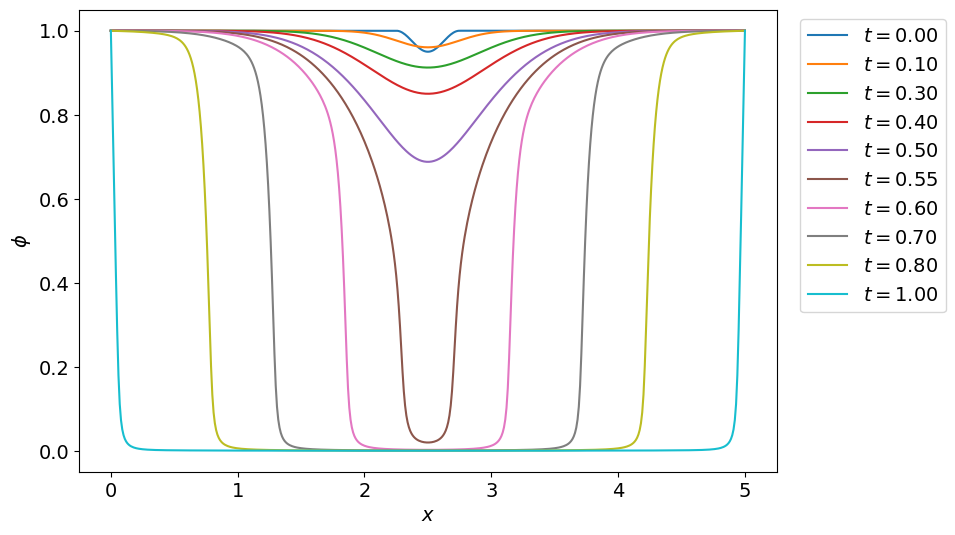
\includegraphics[width=\textwidth]{figures/typical_solution.png}
	\end{figure}
\column{0.12\textwidth}
	\hfill \\
	\vspace{3.5cm}
	\hspace{-2.5cm}
	Узлов по измерениям: \\
	\hspace{-2.5cm}
	$N_x = 10^3$, $N_t = 10^5$
\end{columns}
\end{frame}


\begin{frame}{Результаты: анализ положений равновесия}
\vspace{-0.9cm}
\begin{columns}
\column{0.3\textwidth}
	\begin{center}
		<<Слабое>> напряжение
	\end{center}
	\vspace{-0.2cm}
	$$0 \leqslant \cfrac{K_\Phi^2 l^2 \epsilon_0}{2 \Gamma} < \delta^2$$
	\vspace{-0.7cm}
	\begin{figure}
		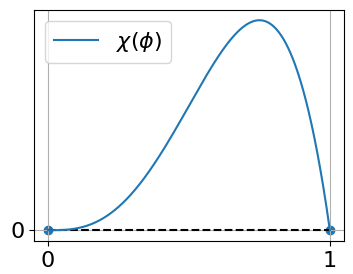
\includegraphics[width=\textwidth]{figures/equilibriums_case_1.png}
	\end{figure}
\column{0.3\textwidth}
	\begin{center}
		<<Среднее>> напряжение
	\end{center}
	\vspace{-0.2cm}
	$$\delta^2 < \cfrac{K_\Phi^2 l^2 \epsilon_0}{2 \Gamma} < (1 + \delta)^2$$
	\vspace{-0.7cm}
	\begin{figure}
		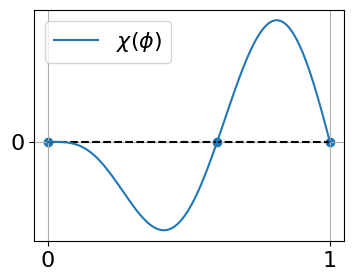
\includegraphics[width=\textwidth]{figures/equilibriums_case_2.png}
	\end{figure}
\column{0.3\textwidth}
	\begin{center}
		<<Сильное>> напряжение
	\end{center}
	\vspace{-0.2cm}
	$$(1 + \delta)^2 < \cfrac{K_\Phi^2 l^2 \epsilon_0}{2 \Gamma}$$
	\vspace{-0.7cm}
	\begin{figure}
		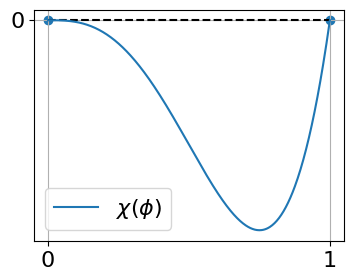
\includegraphics[width=\textwidth]{figures/equilibriums_case_3.png}
	\end{figure}
\end{columns}
\begin{columns}
\column{0.3\textwidth}
	\hspace{0.5cm}
	$\phi \equiv 0$ неустойчивое \\
	\hspace{0.5cm}
	$\phi \equiv 1$ устойчивое
\column{0.3\textwidth}
	\hspace{0.5cm}
	$\phi \equiv 0$ устойчивое \\
	\hspace{0.5cm}
	$\phi \equiv С_3$ неустойчивое \\
	\hspace{0.5cm}
	$\phi \equiv 1$ устойчивое
\column{0.3\textwidth}
	\hspace{0.5cm}
	$\phi \equiv 0$ устойчивое \\
	\hspace{0.5cm}
	$\phi \equiv 1$ неустойчивое
\end{columns}
\end{frame}


\begin{frame}{Результаты: оценка устойчивости}
\vspace{-0.4cm}
\begin{columns}
\column{0.6\textwidth}
	\begin{figure}
		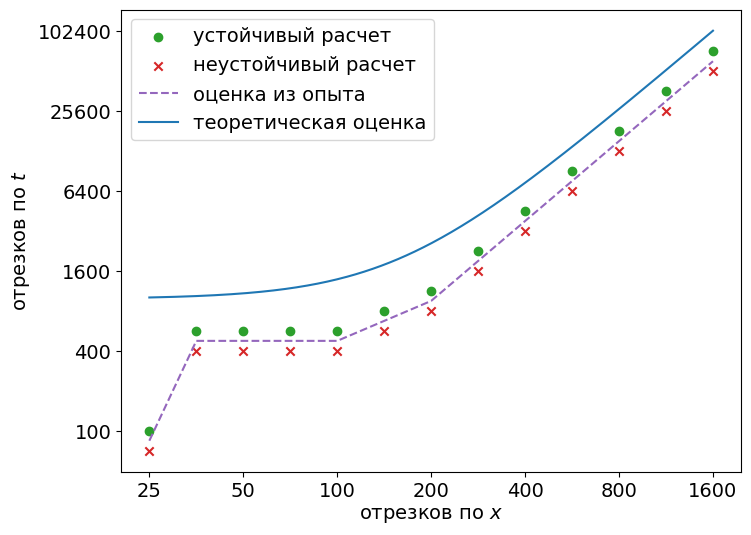
\includegraphics[width=\textwidth]{figures/stability_bounds.png}
	\end{figure}
\column{0.4\textwidth}
	\begin{block}{Условие устойчивости}
		$$\tau \leqslant \cfrac{1}{2m} \left( \cfrac{K_\Phi^2 \epsilon_0}{\delta^{5/3}} + \cfrac{\Gamma}{h^2} \right)^{-1}$$
	\end{block}
\end{columns}
\end{frame}


\begin{frame}{Результаты: исследование обобщения модели}
\begin{itemize}
	\item Поиск стационарного распределения фазового поля вокруг проводников \\ различной конфигурации.
	\item Разностная схема получена методом конечных объемов.
	\item Представление функции-решения в виде ЛК базисных функций позволяет учесть возможную особенность на границе.
\end{itemize}
\end{frame}


\begin{frame}{Работы, готовящиеся к публикации}
\begin{itemize}
	\item Ponomarev A. S., Zipunova E. V., Savenkov E. B. Stability of stationary equilibrium solutions of a diffuse interface electrical breakdown model // Mathematical Models and Computer Simulations. \textcolor{red}{Принято в печать}
	\item Ponomarev A. S., Zipunova E. V. A finite-difference scheme for the generalized diffuse interface model of the electrical breakdown process // Mathematical Models and Computer Simulations. \textcolor{red}{Принято в печать}
	\item Пономарев А. С., Зипунова Е. В., Савенков Е. Б. Устойчивость стационарных решений в модели развития канала электрического пробоя типа <<диффузной границы>> // Препринты ИПМ им. М. В. Келдыша. \textcolor{red}{Направлено в печать}
	\item Пономарев А. С., Зипунова Е. В., Савенков Е. Б. Численное исследование обобщения модели развития канала электрического пробоя типа <<диффузной границы>> // Препринты ИПМ им. М. В. Келдыша. \textcolor{red}{Направлено в печать}
\end{itemize}
\end{frame}


\begin{frame}{Текущая работа}
\begin{itemize}
	\item Разработка алгоритма адаптивного интегрирования по времени.
	\item Настройка параметров модели для воспроизведения результатов \\ физического эксперимента.
\end{itemize}
\end{frame}


\begin{frame}{}
\begin{center}
	\Large
	Спасибо за внимание!
\end{center}
\end{frame}


\end{document}